% Options for packages loaded elsewhere
\PassOptionsToPackage{unicode}{hyperref}
\PassOptionsToPackage{hyphens}{url}
%
\documentclass[
  10pt,
]{article}
\usepackage{amsmath,amssymb}
\usepackage{lmodern}
\usepackage{iftex}
\ifPDFTeX
  \usepackage[T1]{fontenc}
  \usepackage[utf8]{inputenc}
  \usepackage{textcomp} % provide euro and other symbols
\else % if luatex or xetex
  \usepackage{unicode-math}
  \defaultfontfeatures{Scale=MatchLowercase}
  \defaultfontfeatures[\rmfamily]{Ligatures=TeX,Scale=1}
\fi
% Use upquote if available, for straight quotes in verbatim environments
\IfFileExists{upquote.sty}{\usepackage{upquote}}{}
\IfFileExists{microtype.sty}{% use microtype if available
  \usepackage[]{microtype}
  \UseMicrotypeSet[protrusion]{basicmath} % disable protrusion for tt fonts
}{}
\makeatletter
\@ifundefined{KOMAClassName}{% if non-KOMA class
  \IfFileExists{parskip.sty}{%
    \usepackage{parskip}
  }{% else
    \setlength{\parindent}{0pt}
    \setlength{\parskip}{6pt plus 2pt minus 1pt}}
}{% if KOMA class
  \KOMAoptions{parskip=half}}
\makeatother
\usepackage{xcolor}
\IfFileExists{xurl.sty}{\usepackage{xurl}}{} % add URL line breaks if available
\IfFileExists{bookmark.sty}{\usepackage{bookmark}}{\usepackage{hyperref}}
\hypersetup{
  hidelinks,
  pdfcreator={LaTeX via pandoc}}
\urlstyle{same} % disable monospaced font for URLs
\usepackage[margin=1in]{geometry}
\usepackage{longtable,booktabs,array}
\usepackage{calc} % for calculating minipage widths
% Correct order of tables after \paragraph or \subparagraph
\usepackage{etoolbox}
\makeatletter
\patchcmd\longtable{\par}{\if@noskipsec\mbox{}\fi\par}{}{}
\makeatother
% Allow footnotes in longtable head/foot
\IfFileExists{footnotehyper.sty}{\usepackage{footnotehyper}}{\usepackage{footnote}}
\makesavenoteenv{longtable}
\usepackage{graphicx}
\makeatletter
\def\maxwidth{\ifdim\Gin@nat@width>\linewidth\linewidth\else\Gin@nat@width\fi}
\def\maxheight{\ifdim\Gin@nat@height>\textheight\textheight\else\Gin@nat@height\fi}
\makeatother
% Scale images if necessary, so that they will not overflow the page
% margins by default, and it is still possible to overwrite the defaults
% using explicit options in \includegraphics[width, height, ...]{}
\setkeys{Gin}{width=\maxwidth,height=\maxheight,keepaspectratio}
% Set default figure placement to htbp
\makeatletter
\def\fps@figure{htbp}
\makeatother
\setlength{\emergencystretch}{3em} % prevent overfull lines
\providecommand{\tightlist}{%
  \setlength{\itemsep}{0pt}\setlength{\parskip}{0pt}}
\setcounter{secnumdepth}{5}
\usepackage{amsthm}
\usepackage{amsmath}
\usepackage{amssymb}
\usepackage{verbatim}
\usepackage{hyperref}
\usepackage[T1]{fontenc}
\usepackage[utf8]{inputenc}
\hypersetup{colorlinks,allcolors=blue}
\usepackage{enumerate}
\usepackage{lastpage}
\usepackage[shortlabels]{enumitem}
\usepackage{fancyhdr}
\pagestyle{fancy}
\fancyhf{}
\fancyhead[R]{Ingunn Lilja Bergsdóttir}
\fancyhead[C]{Heimaverkefni}
\fancyhead[L]{Hagnýt Bayesísk tölfræði}
\fancyfoot[L]{Háskóli Íslands}
\fancyfoot[R]{\thepage}
\usepackage{float}
\usepackage{algorithm}
\usepackage{algorithmicx}
\usepackage{algpseudocode}
\usepackage{caption}
\usepackage[sectionbib]{chapterbib}
\usepackage{booktabs}
\usepackage{longtable}
\usepackage{array}
\usepackage{multirow}
\usepackage{wrapfig}
\usepackage{float}
\usepackage{colortbl}
\usepackage{pdflscape}
\usepackage{tabu}
\usepackage{threeparttable}
\usepackage{threeparttablex}
\usepackage[normalem]{ulem}
\usepackage{makecell}
\usepackage{xcolor}
\ifLuaTeX
  \usepackage{selnolig}  % disable illegal ligatures
\fi

\author{}
\date{\vspace{-2.5em}}

\begin{document}

\hypertarget{other-exercises-1}{%
\section*{Other exercises 1}\label{other-exercises-1}}
\addcontentsline{toc}{section}{Other exercises 1}

\hypertarget{a}{%
\section*{(a)}\label{a}}
\addcontentsline{toc}{section}{(a)}

Based on Problem 1 in take-home exam from fall 2014 (20\%) In Lieblein and Zelen (1956) data on the endurance of 23 deep groove ball bearings is analyzed. For each of the 23 ball bearings the number of revolutions before failure was collected. The data are inball\_bearings\_data.txt in million revolutions. The data are also shown in the table below,ordered from the smallest value to the largest value.

\begin{center}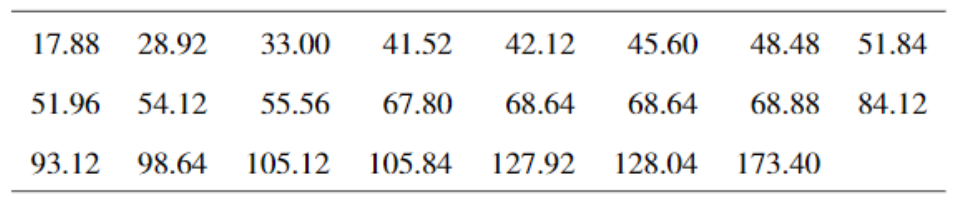
\includegraphics[width=0.75\linewidth]{img/tafla} \end{center}

Let \(y_i\) denote the observed number of revolutions before failure of the i-th ball bearing,
\(i= 1,...,n,(n= 23)\). Assume that they are independent and follow the Rayleigh distribution, such that the density of \(y_i\) is given by.
\[p\left(y_{i} \mid \theta\right)=\theta y_{i} \exp \left(-\frac{\theta y_{i}^{2}}{2}\right), \quad y_{i} \geq 0, \quad i=1, \ldots, n\]

and \(p(y_i|\theta) = 0\) otherwise, where \(\theta\) is an unknown parameter such that \(\theta >0\). Further, assume that the prior density of \(\theta\) is a gamma density with parameters \(\alpha\) and \(\beta\).

\hypertarget{a-1}{%
\section*{(a)}\label{a-1}}
\addcontentsline{toc}{section}{(a)}

Find the posterior distribution of \(\theta\) (with the normalizing constant) in terms of \(\alpha, \beta, y_{1}, \ldots, y_{n}\) Hint:
conjugate distributions.

\hypertarget{b}{%
\section*{(b)}\label{b}}
\addcontentsline{toc}{section}{(b)}

Calculate the mean and standard deviation of the posterior distribution when the observed data areas in the fileball\_bearings\_data.txt and \(\alpha = 1\) and \(\beta= 0.001\).

\hypertarget{c}{%
\section*{(c)}\label{c}}
\addcontentsline{toc}{section}{(c)}

Draw a graph of the posterior density of \(\theta\) using the same data as in (b).

\end{document}
